%%==============================================================
%% Modelo de TCC para o curso de Sistemas de Informação
%% da Universidade Federal de Viçosa - Campus de Rio Paranaíba
%% Autor: Rodrigo Smarzaro (smarzaro@ufv.br)
%% Última versão Agosto/2021
%% Arquivo em formato UTF-8
%% Compilar com pdftex e biber
%% Precisa do arquivo abntex2-UFV.sty
%%==============================================================

\documentclass[
    % -- opções da classe memoir --
    12pt,                   % tamanho da fonte
    openright,              % capítulos começam em página ímpar (insere página vazia caso preciso)
    oneside,                % para impressão só no anverso. Oposto a twoside
    a4paper,                % tamanho do papel.
    % -- opções do pacote abntex2 --
    % chapter=TITLE,        % Títulos em maiúsculas
    sumario=tradicional,    % Sumário padrão memoir 
    % -- opções do pacote babel --
    english,                % idioma adicional para hifenização
    brazil,                 % idioma principal do documento
    ]{abntex2}

% Pacotes fundamentais
\usepackage{abntex2-UFV}        % Personalização para a Universidade Federal de Viçosa
\usepackage{lmodern}            % Usa a fonte Latin Modern
\usepackage[T1]{fontenc}        % Seleção de códigos de fonte de saída
\usepackage[utf8]{inputenc}        % Codificação do documento (conversão automática dos acentos)
\usepackage{indentfirst}        % Indenta o primeiro parágrafo de cada seção.
\usepackage{graphicx}            % Inclusão de gráficos
\usepackage{booktabs}           % \toprule, \midrule e \bottomrule para tabelas
\usepackage{csquotes}
\usepackage[final]{microtype} 			% para melhorias de justificação
\usepackage{hyphenat}
\usepackage{tikz}              % Figura da arquitetura do protótipo
\usetikzlibrary{arrows.meta,positioning,calc}




% Sistema autor-data com títulos nas referências em negrito
%\usepackage[alf,abnt-emphasize=bf]{abntex2cite}

% uso do biblatex, mais flexível e moderno
\usepackage[backend=biber,
            style=abnt,
            uniquename=init,
            giveninits,
            repeatfields,
            justify,
            noslsn]{biblatex}

\usepackage{xurl}
\urlstyle{same}

\addbibresource{referencias.bib}


%\PassOptionsToPackage{hyphens}{url}\usepackage{hyperref}
%\usepackage{url}
% permitir quebra de linha em URLs
%\makeatletter
%\g@addto@macro{\UrlBreaks}{\UrlOrds}
%\makeatother

\setlength\bibparsep{10pt}

% ---
% CONFIGURAÇÕES DE PACOTES
% ---

% Informações de dados para CAPA e FOLHA DE ROSTO
\titulo{Geração de Explicações de Código Baseadas em Inteligência Artificial com Foco na Identificação de Pontos Críticos e Alinhamento à Regra de Negócio para Programadores com Deficiência Visual}
\autor{João Pedro Silva Coelho}
\local{Rio Paranaíba}
\data{2026}
\orientador{Adriana Zanella Martinhago}    % redefinido no abntex2-UFV para aceitar Instituição (default = UFV-CRP)
%\coorientador{Nome do Coorientador}
\instituicao{Universidade Federal de Viçosa}

\campus{\emph{Campus} Rio Paranaíba}      % pacote abntex2-UFV
\curso{Sistemas de Informação}               % pacote abntex2-UFV
\membrobancaA{Membro da Banca A}             % pacote abntex2-UFV default = UFV-CRP
\membrobancaB{Membro da Banca B}       % pacote abntex2-UFV default = UFV-CRP
\databanca{\today}                           % pacote abntex2-UFV

% O preambulo deve conter o tipo do trabalho, o objetivo,
% o nome da instituição e a área de concentração
\preambulo{Monografia apresentada à Universidade Federal de Viçosa, como parte das exigências para a aprovação na disciplina Trabalho de Conclusão de Curso I}
% ---

% ---
% Configurações de aparência do PDF final

% informações para o arquivo pdf de saída
% Interessante alterar a cor dos links para preto(black)
% na versão final para imprimir
\makeatletter
\hypersetup{
        % metadados
        pdftitle={\@title},
        pdfauthor={\@author},
        pdfsubject={\imprimirpreambulo},
        pdfcreator={LaTeX with abnTeX2},
        colorlinks=true,   % false: links em frame; true: links coloridos
        linkcolor=black,   % cor dos links no documento
        citecolor=blue,    % cor dos links para a bibliografia
        filecolor=magenta, % cor dos links para arquivos
        urlcolor=blue,     % cor dos links para sites
        bookmarksdepth=4   % profundidade do sumário do PDF
}
\makeatother
% ---

\begin{document}
% Retira espaço extra obsoleto entre as frases.
\frenchspacing

% ----------------------------------------------------------
% ELEMENTOS PRÉ-TEXTUAIS
% ----------------------------------------------------------
\pretextual

% Capa
\imprimircapa

% Folha de rosto
\imprimirfolhaderosto
% ---

% Inserir folha de aprovação
% \imprimirfolhadeaprovacao

% Dedicatória
% \begin{dedicatoria}
%    \vspace*{\fill}
%    \centering
%    \noindent
%    \textit{Texto qualquer da dedicatória}
%    \vspace*{\fill}
% \end{dedicatoria}
% ---

% Agradecimentos
% \begin{agradecimentos}
% %Insira o texto de agradecimentos aqui
% \end{agradecimentos}
% ---

% Epígrafe
% \begin{epigrafe}
%     \vspace*{\fill}
%     \begin{flushright}
%         \textit{``Word? nunca mais.''\\
%         (Qualquer usuário de \LaTeX)}
%     \end{flushright}
% \end{epigrafe}
% ---

% RESUMOS

% resumo em português
\begin{resumo}
 \noindent
 %Insira o resumo aqui
 A programação envolve processos cognitivos complexos, especialmente no que se refere à compreensão da lógica e das regras de negócio presentes no código-fonte. Para programadores com deficiência visual, essa compreensão depende de tecnologias assistivas, como os leitores de tela, cujas limitações no acesso à estrutura do código e à saída das ferramentas de desenvolvimento são relatadas na literatura. Embora avanços recentes em Inteligência Artificial tenham ampliado as possibilidades de geração e explicação de código, essas soluções, em geral, não são projetadas considerando requisitos de acessibilidade na forma de entrega das explicações. Este trabalho desenvolve e avalia tecnicamente um protótipo, escrito em Python, que combina a análise estática do código-fonte, para a identificação de pontos críticos do código, com modelos de linguagem de grande porte, executados localmente ou em nuvem, para a geração de explicações estruturadas alinhadas à regra de negócio. As explicações são entregues como texto e vocalizadas pelo leitor de tela NVDA. A validação compreende testes automatizados, a verificação da integração com o NVDA e a comparação entre modelos segundo critérios de acessibilidade; a avaliação com programadores com deficiência visual é proposta por meio de um protocolo exploratório e discutida como limitação.
 \vspace{\onelineskip}

 \noindent
 \textbf{Palavras-chave}: Acessibilidade, Inteligência Artificial, Compreensão de Código, Leitores de Tela
\end{resumo}

% resumo em inglês
\begin{resumo}[Abstract]
\begin{otherlanguage*}{english}
  \noindent
  %Insira o abstract aqui
  Programming involves complex cognitive processes, particularly with regard to understanding the logic and business rules embedded in source code. For programmers with visual impairments, this understanding depends on assistive technologies such as screen readers, whose limitations in conveying code structure and the output of development tools are reported in the literature. Although recent advances in Artificial Intelligence have expanded the possibilities for code generation and explanation, these solutions are generally not designed with accessibility requirements for the delivery of explanations in mind. This work develops and technically evaluates a prototype, written in Python, that combines static analysis of source code, to identify critical points in the code, with large language models, run locally or in the cloud, to generate structured explanations aligned with business rules. The explanations are delivered as text and spoken by the NVDA screen reader. Validation comprises automated tests, verification of the integration with NVDA, and a comparison of models according to accessibility criteria; an evaluation with programmers with visual impairments is proposed as an exploratory protocol and discussed as a limitation.
  \vspace{\onelineskip}

  \noindent
  \textbf{Keywords}: Accessibility, Artificial Intelligence, Code Comprehension, Screen Readers
 \end{otherlanguage*}
\end{resumo}

% inserir lista de ilustrações
\pdfbookmark[0]{\listfigurename}{lof}
\listoffigures*
\cleardoublepage
% ---

% inserir lista de tabelas
% \pdfbookmark[0]{\listtablename}{lot}
% \listoftables*
\cleardoublepage
% ---

% Lista de siglas e abreviaturas (opcional)
% sintaxe: \item [sigla] Descrição da sigla

%\begin{siglas}
%\item[ABNT] Absurdas Normas Técnicas
%\item[UFV] Universidade Federal de Viçosa
%\item[CRP] \emph{Campus} de Rio Paranaíba
%\end{siglas}

% Lista de símbolos (opcional)
% sintaxe: \item [simbolo] Descrição do símbolo

%\begin{simbolos}
%\item[$\infty$ ] Infinito
%\end{simbolos}

% inserir o sumario
\pdfbookmark[0]{\contentsname}{toc}
\tableofcontents*
\cleardoublepage
% ---

% ----------------------------------------------------------
% ELEMENTOS TEXTUAIS
% ----------------------------------------------------------
\textual

%Modifique a estrutura dos capítulos e seções de acordo com a necessidade do seu trabalho
\chapter{Introdução}\label{sec:introducao}

A Tecnologia da Informação ocupa um papel cada vez mais relevante na sociedade contemporânea, tornando o desenvolvimento de software uma atividade estratégica em diversos contextos. Nesse cenário, pesquisas têm investigado as dificuldades enfrentadas por pessoas com deficiência visual na programação e nos ambientes de desenvolvimento \cite{acad54431201,latinoware20457}.

\textcite{latinoware20457} aplicaram um questionário a dez desenvolvedores com deficiência visual e avaliaram, com verificadores automáticos de acessibilidade, quatro ferramentas utilizadas no desenvolvimento de software; os respondentes relataram dificuldades como a navegação entre os arquivos de um projeto, a depuração de programas e a localização de erros de sintaxe. Em um estudo de caso em uma disciplina de programação, \textcite{acad54431201} observaram que o leitor de tela, isoladamente, não é suficiente para compreender a estrutura do código e que as mensagens de erro de compilação exibidas em um painel da IDE não eram lidas. Esses resultados reforçam a importância de soluções que auxiliem não apenas a edição do código, mas também a sua interpretação.

Os leitores de tela, embora fundamentais para a acessibilidade digital, apresentam a informação de forma sequencial, pela fala, o que torna custoso reconstruir mentalmente a organização de um programa e localizar os trechos que concentram regras de negócio ou risco; essa é a premissa de projeto adotada neste trabalho. Para ambientes de desenvolvimento web, \textcite{latinoware6969} constataram, em testes com o NVDA, que as ferramentas avaliadas não anunciam erros de sintaxe ao leitor de tela e que a saída do terminal é inacessível ou apenas parcialmente acessível.

Paralelamente, os modelos de linguagem de grande porte vêm sendo aplicados a diversas tarefas da Engenharia de Software \cite{hou2024llmse} e já chegam aos ambientes utilizados por programadores com deficiência visual. \textcite{latinoware34224} investigaram o uso de ferramentas de Inteligência Artificial por programadores cegos e registraram ganhos de produtividade e de confiança, mas também que as sugestões de código exibidas na tela não eram lidas pelo leitor de tela, o que obrigava os participantes a explorar a interface manualmente para localizá-las. Esse achado indica que a forma de entrega da saída da Inteligência Artificial é, por si só, uma barreira de acessibilidade.

Além disso, entre os trabalhos analisados, grande parte concentra-se na adaptação de interfaces e no suporte ao uso de ambientes de desenvolvimento. \textcite{latinoware37693}, por exemplo, propõem diretrizes de acessibilidade para ambientes de desenvolvimento integrado, enquanto \textcite{latinoware40920} apresentam uma ferramenta voltada à construção acessível de páginas web por programadores cegos ou com baixa visão. Permanece, portanto, uma lacuna no uso de recursos capazes de explicar o código-fonte já existente, destacando seus pontos críticos e relacionando-os à regra de negócio, em um formato adequado à escuta por leitores de tela.

Diante desse cenário, este trabalho propõe e implementa um protótipo, escrito em Python, que combina a análise estática do código-fonte, responsável por identificar os pontos críticos do código de forma determinística, com modelos de linguagem de grande porte, responsáveis por redigir explicações estruturadas alinhadas à regra de negócio. As explicações seguem regras de acessibilidade definidas no trabalho, como frases curtas, ausência de tabelas e de símbolos decorativos e marcação explícita do que é dedução, e são entregues ao programador por meio do leitor de tela NVDA.

O restante deste documento está organizado da seguinte forma. O Capítulo~\ref{sec:refteorico} apresenta o referencial teórico sobre acessibilidade na programação, leitores de tela, modelos de linguagem de grande porte, engenharia de prompts e prototipação. O Capítulo~\ref{sec:TrabRel} discute os trabalhos relacionados. O Capítulo~\ref{sec:metodos} descreve os métodos, incluindo a arquitetura do protótipo, a seleção dos modelos de linguagem e a estratégia de validação. O Capítulo~\ref{sec:resultEsperados} apresenta os resultados parciais e os resultados esperados, o Capítulo~\ref{sec:limitacoes} discute as limitações e os trabalhos futuros e o Capítulo~\ref{sec:cronograma} apresenta o cronograma e a análise de exequibilidade.

\section{Objetivos}\label{sec:objetivos}

\subsection{Objetivo Geral}

Desenvolver e avaliar tecnicamente um protótipo baseado em Inteligência Artificial que gere explicações estruturadas de código-fonte Python, com foco na identificação de pontos críticos e no alinhamento à regra de negócio, e as entregue a programadores com deficiência visual por meio de leitores de tela.

\subsection{Objetivos Específicos}

\begin{itemize}
  \item Realizar revisão e análise da literatura sobre acessibilidade, tecnologias assistivas, modelos de linguagem de grande porte e engenharia de prompts aplicados à compreensão de código-fonte.
  \item Definir os requisitos funcionais, os requisitos não funcionais e os critérios para a identificação de pontos críticos no código-fonte.
  \item Definir uma estrutura de explicação acessível, compatível com leitores de tela e alinhada à compreensão de regras de negócio.
  \item Desenvolver um protótipo capaz de analisar um projeto Python, identificar pontos críticos por meio de regras determinísticas e gerar explicações por meio de modelos de linguagem executados localmente ou em nuvem.
  \item Selecionar modelos de linguagem candidatos, justificando a escolha, e compará-los segundo a conformidade com as regras de acessibilidade, a cobertura dos pontos críticos e o custo computacional.
  \item Validar tecnicamente a integração do protótipo com o leitor de tela NVDA e a conformidade das explicações com as regras de acessibilidade definidas.
  \item Elaborar um protocolo de avaliação com programadores com deficiência visual e, se viável no prazo do trabalho, aplicá-lo de forma exploratória, discutindo as limitações de uma validação exclusivamente técnica.
\end{itemize}


\chapter{Referencial Teórico}\label{sec:refteorico}

O referencial teórico deste trabalho está fundamentado em estudos sobre acessibilidade computacional, programação por pessoas com deficiência visual, leitores de tela, modelos de linguagem de grande porte, engenharia de prompts e prototipação. A integração desses temas permite compreender os desafios enfrentados por programadores com deficiência visual e fundamentar as escolhas técnicas do protótipo, em especial a seleção dos modelos de linguagem e o desenho dos \textit{prompts}.

\section{Acessibilidade na programação}\label{sec:AcessComputacao}

A acessibilidade na computação diz respeito à possibilidade de que sistemas, ferramentas e tecnologias sejam utilizados de forma autônoma por diferentes perfis de usuários, incluindo pessoas com deficiência. Na Engenharia de Software, esse conceito não se restringe às aplicações destinadas ao usuário final, pois alcança também os ambientes e as ferramentas empregados no próprio desenvolvimento, como mostram os trabalhos que investigam ambientes de desenvolvimento acessíveis \cite{latinoware37693,latinoware6969}.

As diretrizes WCAG (\textit{Web Content Accessibility Guidelines}) organizam-se em quatro princípios: perceptível, operável, compreensível e robusto \cite{w3c2024wcag22}. Embora tenham sido propostas para o conteúdo web, \textcite{latinoware6969} utilizam as diretrizes WCAG, juntamente com as diretrizes WAI-ARIA, UAAG e ATAG, como critérios técnicos para avaliar a acessibilidade de ambientes de desenvolvimento, verificando se as ferramentas são perceptíveis, operáveis e compatíveis com o leitor de tela NVDA.

Os estudos analisados indicam que muitas ferramentas de desenvolvimento ainda apresentam barreiras relacionadas à navegação, ao retorno de informações ao leitor de tela e à interação com tecnologias assistivas. \textcite{latinoware20457} registraram, entre os respondentes com deficiência visual, dificuldades de navegação entre arquivos, de depuração e de localização de erros de sintaxe. \textcite{acad54431201} observaram que o leitor de tela, isoladamente, não permite compreender a estrutura do código, pois a indentação não é transmitida pela fala, e que os erros de compilação apresentados em um painel da IDE não eram lidos. \textcite{latinoware34224} constataram que as sugestões geradas por ferramentas de Inteligência Artificial, exibidas na tela, não eram vocalizadas, e \textcite{latinoware6969} verificaram que erros de sintaxe não são anunciados e que a saída do terminal é inacessível ou apenas parcialmente acessível.

Dessa forma, promover a acessibilidade na programação não significa apenas adaptar interfaces existentes, mas também apresentar a informação de maneira estruturada e em formato adequado à escuta. Essa perspectiva abre espaço para o emprego da Inteligência Artificial na geração de explicações acessíveis e no apoio à compreensão de código-fonte por programadores com deficiência visual, tema central desta pesquisa.

\section{Tecnologias Assistivas e Leitores de Tela}\label{sec:TecAssistivas}

As tecnologias assistivas desempenham papel fundamental na promoção da acessibilidade digital para pessoas com deficiência visual. Entre elas, os leitores de tela são os recursos de uso mais frequente: na pesquisa de \textcite{latinoware20457}, a maioria dos respondentes com deficiência visual declarou utilizar um leitor de tela. Esses programas interpretam as informações exibidas pelo sistema operacional e as apresentam em saída sonora, por meio de voz sintetizada, ou tátil, por meio de displays Braille \cite{nvaccess2026guia}.

O NVDA (\textit{NonVisual Desktop Access}) é um leitor de tela gratuito e de código aberto para o sistema operacional Windows, desenvolvido pela NV Access \cite{nvaccess2026guia}. Na pesquisa de \textcite{latinoware20457}, foi o leitor de tela mais citado pelos respondentes (cinco dos que declararam usar leitor de tela), e \textcite{latinoware6969} o adotaram como leitor de tela nos testes de acessibilidade de ambientes de desenvolvimento. Por essa combinação de gratuidade, uso entre o público-alvo e disponibilidade de uma interface para integração com outros programas, o NVDA foi escolhido como leitor de tela de referência para o protótipo.

O NVDA oferece suporte às interfaces de acessibilidade \textit{Microsoft Active Accessibility} (MSAA), \textit{IAccessible2} (IA2), \textit{UI Automation} (UIA) e \textit{Java Access Bridge}, que lhe permitem obter informações dos aplicativos. Para documentos e páginas web, disponibiliza o modo de navegação (\textit{browse mode}), no qual o usuário percorre o conteúdo com teclas de atalho que saltam entre títulos, \textit{links}, campos de formulário e outros elementos; a saída é apresentada por sintetizadores de voz, como o eSpeak NG e as vozes SAPI e OneCore, e por displays Braille \cite{nvaccess2026guia}. A Figura~\ref{fig:ciclo-nvda} resume esse funcionamento: um evento do sistema operacional, como o pressionamento de uma tecla ou a mudança de foco, é capturado por APIs de acessibilidade; o leitor de tela identifica o tipo de conteúdo, utilizando o modo de navegação para páginas web e documentos ou acessando diretamente os elementos da interface em aplicações desktop; e as informações processadas são apresentadas por sintetizador de voz ou display Braille, quando disponível. O ciclo se repete a cada novo evento gerado pelo sistema.

\begin{figure}[htbp]
  \centering
  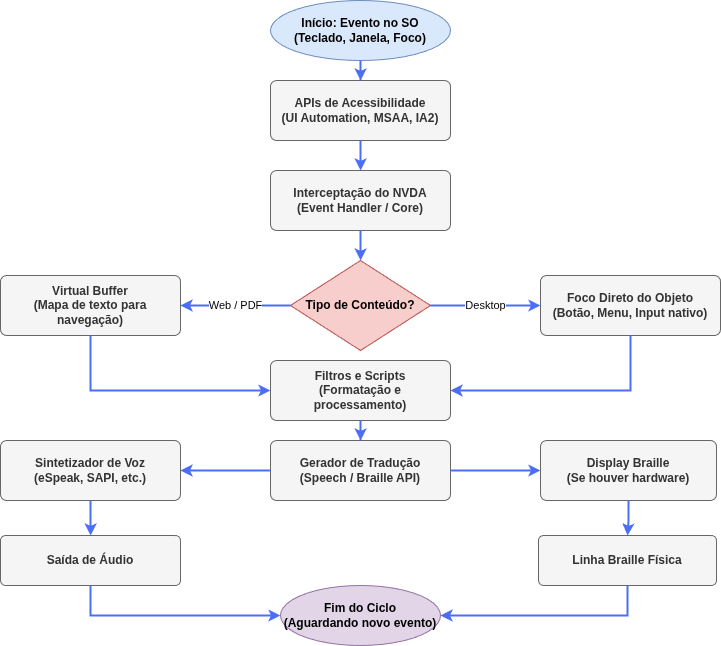
\includegraphics[width=.7\linewidth]{fluxograma_NVDA.png}
  \caption{Diagrama simplificado do ciclo de execução de um leitor de tela, evidenciando a captura de eventos por APIs de acessibilidade (MSAA, UIA, IA2), a divisão do processamento por tipo de conteúdo (\textit{Buffer Virtual} e Foco Direto) e as interfaces de saída de áudio e Braille}
  \legend{Fonte: Elaborado pelo autor.}
  \label{fig:ciclo-nvda}
\end{figure}

Embora o NVDA represente uma ferramenta essencial para a inclusão digital, os estudos apontam limitações importantes no contexto da programação. Os erros de sintaxe e de compilação nem sempre são anunciados ou lidos \cite{latinoware6969,acad54431201}, a saída do terminal pode ser inacessível \cite{latinoware6969} e a estrutura do código, como a indentação, não é transmitida pela fala \cite{acad54431201}. Essas limitações justificam a busca por formas complementares de apresentar ao usuário a organização do código e os trechos que merecem atenção.

Além de ler a interface, o NVDA pode receber texto de outros programas. A biblioteca \textit{NVDA Controller Client} é uma biblioteca de vínculo dinâmico (DLL) que permite a um aplicativo solicitar ao NVDA que fale um texto ou o exiba em Braille, podendo ser chamada de qualquer linguagem capaz de invocar símbolos de uma DLL, como o Python por meio do módulo \textit{ctypes} \cite{nvaccess2024controller}. A documentação da biblioteca recomenda que o aplicativo verifique se o Windows está bloqueado ou em tela segura antes de enviar informações ao usuário, pois o NVDA também opera nessas telas \cite{nvaccess2024controller}. É por meio dessa biblioteca que o protótipo entrega as explicações ao programador.

\section{Inteligência Artificial e Modelos de Linguagem}\label{sec:IA}

Entre as abordagens de Inteligência Artificial com maior aplicação recente na Engenharia de Software destacam-se os modelos de linguagem de grande porte (\textit{Large Language Models} -- LLMs) \cite{hou2024llmse}. Esta seção apresenta os fundamentos desses modelos, as características dos modelos de pesos abertos que podem ser executados localmente, as técnicas de engenharia de \textit{prompts} empregadas para controlá-los e as principais aplicações à compreensão de código-fonte.

\subsection{Modelos de Linguagem de Grande Porte}\label{sec:LLM}

A arquitetura \textit{Transformer}, proposta por \textcite{vaswani2017attention}, dispensa recorrência e convoluções e se baseia exclusivamente em mecanismos de atenção, o que favorece a paralelização do treinamento. Modelos de grande porte, como o Llama~3, cujo maior modelo é um \textit{Transformer} denso com 405 bilhões de parâmetros e janela de contexto de até 128 mil \textit{tokens} \cite{grattafiori2024llama3}, exemplificam o emprego dessa arquitetura em larga escala.

\textcite{brown2020fewshot} mostraram, com o GPT-3, de 175 bilhões de parâmetros, que o aumento de escala melhora substancialmente a capacidade de o modelo executar novas tarefas de linguagem a partir de poucos exemplos ou de instruções em linguagem natural, sem ajuste fino. \textcite{ouyang2022instructions} observaram, por sua vez, que o aumento de escala, por si só, não faz o modelo seguir a intenção do usuário, e que o ajuste com supervisão e com aprendizado por reforço a partir de realimentação humana produziu um modelo de 1,3 bilhão de parâmetros cujas respostas foram preferidas pelos avaliadores às do GPT-3 de 175 bilhões; os autores registram, porém, que os modelos ainda cometem erros simples.

No domínio do código-fonte, \textcite{chen2021codex} apresentam o Codex, modelo derivado do GPT e treinado adicionalmente com código público do GitHub, avaliado no \textit{benchmark} HumanEval, que verifica se programas gerados a partir de descrições (\textit{docstrings}) funcionam corretamente; os autores também relatam limitações, como a dificuldade com longas cadeias de operações. A revisão sistemática de \textcite{hou2024llmse}, que analisou 395 trabalhos publicados entre 2017 e o início de 2024, mapeou quais modelos são empregados, em quais tarefas de Engenharia de Software e como seu desempenho é otimizado e avaliado.

Nesses estudos, o foco recai sobre a correção e a cobertura de tarefas de programação, e não sobre a forma como o texto produzido é recebido por usuários de leitores de tela. Por essa razão, neste trabalho o modelo de linguagem é utilizado como redator de explicações, enquanto a identificação dos pontos críticos do código permanece a cargo da análise estática (Seção~\ref{sec:prototipo}), e a forma do texto é controlada por regras explícitas no \textit{prompt} (Seção~\ref{sec:estrategia}).

\subsection{Modelos Abertos, Execução Local e Janela de Contexto}\label{sec:modelosabertos}

Além dos modelos acessíveis apenas por meio de serviços de terceiros, há famílias de modelos com pesos disponibilizados publicamente, que podem ser executadas em equipamento próprio. O Qwen3, por exemplo, reúne modelos densos e de mistura de especialistas de 0,6 a 235 bilhões de parâmetros, é distribuído sob a licença Apache~2.0, amplia o suporte de 29 para 119 idiomas e dialetos e integra, em um único modelo, os modos de raciocínio e de resposta rápida \cite{yang2025qwen3}. O GPT-OSS, primeira família de pesos abertos da OpenAI desde o GPT-2, foi avaliado por \textcite{bi2025gptoss}, que o consideraram relativamente forte na geração de código e mais fraco em tarefas multilíngues, o que é relevante para explicações em português. A página do Gemma~4, do Google DeepMind, na biblioteca do Ollama descreve versões que variam de 2 bilhões (parâmetros efetivos) a 31 bilhões de parâmetros, com janelas de contexto de 128 mil a 256 mil \textit{tokens}, modos de raciocínio configuráveis e uma variante hospedada em nuvem \cite{ollama2026gemma4}. Já o GPT-4o, modelo multimodal da OpenAI, é descrito como equivalente ao GPT-4 Turbo em texto e código em inglês e como mais rápido e mais barato na API \cite{openai2024gpt4o}.

O Ollama permite executar esses modelos localmente e também acessar modelos hospedados em seus servidores por meio de uma chave de API; nesse caso, segundo a documentação, os \textit{prompts} e as respostas são processados apenas para atender às requisições e não são utilizados para treinar modelos \cite{ollama2026nuvem}. A execução local mantém o código analisado no equipamento do usuário, ao passo que o uso da nuvem o transmite a terceiros, o que precisa ser considerado ao analisar código privado.

A janela de contexto limita a quantidade de texto, medida em \textit{tokens}, que o modelo recebe de uma vez. No Ollama, o tamanho padrão depende da memória de vídeo disponível: cerca de 4 mil \textit{tokens} com menos de 24~GiB, 32 mil entre 24 e 48~GiB e 256 mil com 48~GiB ou mais, enquanto os modelos em nuvem utilizam o contexto máximo \cite{ollama2026contexto}. Em equipamentos com menos de 24~GiB, portanto, o contexto padrão é pequeno, e o seu tamanho precisa ser configurado explicitamente para que o código de projetos reais caiba na requisição.

\subsection{Engenharia de Prompts}\label{sec:prompts}

A engenharia de \textit{prompts} consiste em fornecer ao modelo instruções de tarefa, em linguagem natural ou por vetores aprendidos, sem alterar seus parâmetros \cite{sahoo2024prompt}. \textcite{sahoo2024prompt} organizam as técnicas em uma taxonomia por área de aplicação, apresentando, para cada uma, a abordagem, os modelos e os conjuntos de dados empregados e seus pontos fortes e limitações. Entre as técnicas descritas na literatura estão o fornecimento de poucos exemplos no próprio \textit{prompt} \cite{brown2020fewshot} e o encadeamento de raciocínio (\textit{chain-of-thought}), em que os exemplos incluem os passos intermediários da solução, associado por \textcite{wei2022cot} a ganhos em tarefas aritméticas, de senso comum e simbólicas.

Para explicações destinadas à escuta, a engenharia de \textit{prompts} assume uma função adicional: além de orientar o conteúdo, precisa impor a forma do texto, pois quem ouve a explicação não pode retornar a um trecho nem distinguir visualmente fatos de suposições. Por isso, o protótipo emprega instruções diretas, sem exemplos, que combinam regras de conteúdo e regras de forma, e fornece ao modelo dados já extraídos pela análise estática, de modo que ele explique o que foi encontrado em vez de decidir o que é crítico (Seção~\ref{sec:estrategia}). Como o ajuste de modelos para seguir instruções melhora, mas não elimina, falhas de obediência \cite{ouyang2022instructions}, a verificação automática do texto produzido integra a validação do protótipo (Seção~\ref{sec:validacao}).

\subsection{Inteligência Artificial Aplicada à Engenharia de Software}\label{sec:IAES}

Na Engenharia de Software, os modelos de linguagem têm sido aplicados a tarefas diversas, o que motivou revisões sistemáticas da área \cite{hou2024llmse}. No estudo de \textcite{latinoware34224}, programadores cegos utilizaram ferramentas como o ChatGPT para corrigir e aprimorar código, gerar código, completar trechos e localizar e explicar erros, e relataram aumento de produtividade e de confiança.

A sumarização automática de código, isto é, a geração de descrições em linguagem natural a partir do código-fonte, é uma das tarefas investigadas. \textcite{sun2023chatgptsum} avaliaram o ChatGPT nessa tarefa, comparando-o com modelos de referência (NCS, CodeBERT e CodeT5) segundo as métricas BLEU, METEOR e ROUGE-L, e observaram desempenho inferior ao desses modelos em BLEU e ROUGE-L. Essas métricas comparam o texto gerado com comentários de referência por sobreposição de palavras e, por isso, não verificam se a descrição é adequada à escuta por leitor de tela nem se ajuda a compreender regras de negócio. Essa lacuna justifica a definição, neste trabalho, de critérios próprios de verificação das explicações (Seção~\ref{sec:validacao}).

Além disso, a forma de entrega da saída dos assistentes de Inteligência Artificial ainda é uma barreira: \textcite{latinoware34224} constataram que as sugestões exibidas no editor não eram vocalizadas pelo leitor de tela e propuseram, entre outras melhorias, sinais sonoros ou mensagens quando um código é gerado. Nesse contexto, a combinação de modelos de linguagem, identificação de pontos críticos do código e geração de explicações semanticamente estruturadas apresenta-se como uma oportunidade de pesquisa, que este trabalho explora.

\section{Prototipação}\label{sec:Prototipacao}

A prototipação é uma técnica amplamente empregada no desenvolvimento de software. Segundo \textcite{latinoware7985}, um protótipo é uma versão preliminar de um sistema, utilizada para demonstrar conceitos, testar alternativas de projeto e compreender melhor o problema; entre os benefícios descritos estão validar cedo o projeto e a usabilidade, obter retorno dos usuários, esclarecer requisitos, reduzir o risco de mudanças de requisitos, melhorar a comunicação entre as partes interessadas e avaliar alternativas a baixo custo.

Os autores distinguem protótipos de baixa e de alta fidelidade. Os de baixa fidelidade, como esboços e modelos em papel, exigem menos preparo e são mais fáceis de alterar durante os testes; os de alta fidelidade, em geral construídos com ferramentas digitais, oferecem interação mais realista e permitem avaliar fluxos de trabalho e detalhes visuais \cite{latinoware7985}. Em uma revisão rápida de 30 estudos primários, \textcite{latinoware7985} não identificaram estudos que investiguem a prototipação para a validação de acessibilidade, o que indica espaço para trabalhos como este.

O estudo de \textcite{latinoware7985} trata de protótipos de interface do usuário. O protótipo desenvolvido neste trabalho, por sua vez, não é uma interface gráfica, mas uma ferramenta funcional executada em linha de comando, cuja saída é textual e sonora; sua fidelidade, portanto, refere-se ao comportamento funcional (análise, geração e fala), e não ao aspecto visual. Ele foi construído de forma incremental, em fases, o que permite validar cada etapa antes de acrescentar a seguinte (Seção~\ref{sec:prototipo}).


\chapter{Trabalhos Relacionados}\label{sec:TrabRel}

O presente trabalho situa-se na interseção entre Inteligência Artificial, Engenharia de Software e acessibilidade. Para contextualizar e fundamentar a proposta, foram analisados trabalhos que abordam o uso de ferramentas de Inteligência Artificial por programadores com deficiência visual, a acessibilidade de ambientes de desenvolvimento e a sumarização automática de código com modelos de linguagem. A seguir, são apresentados quatro trabalhos que estabelecem uma base para a compreensão e o desenvolvimento da ferramenta proposta, seguidos de uma síntese que posiciona esta proposta em relação a eles.

\section{Inteligência Artificial e Acessibilidade: Uma Experiência de Inclusão para Programadores Cegos em Ambientes de Desenvolvimento}

\textcite{latinoware34224} investigaram como ferramentas de Inteligência Artificial podem tornar o ensino de programação mais acessível e eficiente para estudantes cegos. Participaram quatro programadores totalmente cegos, em sessões remotas, que resolveram o mesmo exercício de ordenação com e sem o apoio de Inteligência Artificial, em ambientes como o \textit{VS Code} e o \textit{Repl.it}, e foram entrevistados e responderam a questionários. Os resultados indicaram que a Inteligência Artificial corrigiu erros em segundos e aumentou a produtividade e a confiança dos participantes, mas também que as sugestões exibidas na tela não eram lidas pelo leitor de tela, que a localização das sugestões e a revisão da saída do terminal eram difíceis e que elementos gráficos das IDEs dificultavam o uso.

Entre as limitações, a amostra é muito pequena, a análise é predominantemente qualitativa e o artigo não informa as versões nem as configurações dos modelos utilizados, o que dificulta a reprodução. Ainda assim, ao apontar que a forma de entrega das sugestões é uma barreira e ao propor sinais sonoros ou mensagens quando um código é gerado, o trabalho fundamenta o requisito deste TCC de que as explicações sejam entregues em texto adequado à escuta e vocalizadas pelo leitor de tela, em vez de dependerem da exploração visual ou manual da tela. O procedimento de comparação com e sem Inteligência Artificial também inspira o protocolo de avaliação com usuários proposto na Seção~\ref{sec:usuarios}.

\section{WAE - Web Accessibility Engine: Uma Ferramenta de Transpilação Acessível e Estruturada para Programadores Cegos ou de Baixa Visão}

\textcite{latinoware40920} apresentam o WAE (\textit{Web Accessibility Engine}), ferramenta desenvolvida para facilitar a prototipação e a construção de páginas web estáticas por programadores cegos ou com baixa visão. A pesquisa incluiu uma revisão da literatura que levou à escolha do paradigma de codificação acessível \textit{Grid Coding} e da linguagem YAML como bases do projeto. A acessibilidade das páginas geradas foi avaliada com o Avaliador e Simulador de Acessibilidade em Sítios (ASES), e os autores reportam que a maioria dos componentes criados pelo WAE atendeu a altos padrões de acessibilidade, o que indica o potencial da ferramenta para o desenvolvimento web inclusivo.

O trabalho é relevante para esta pesquisa por abordar ferramentas que promovem a acessibilidade no desenvolvimento de software por meio de paradigmas de codificação estruturados, aproximando-se do objetivo de gerar explicações estruturadas e semanticamente orientadas. Por outro lado, o resumo do artigo não descreve avaliação com usuários nem apresenta valores numéricos para os resultados do ASES, e a ferramenta é voltada à produção de páginas web, e não à explicação de código existente. Como o ASES avalia páginas web, ele também não se aplica diretamente a explicações em texto; por isso, este trabalho define critérios próprios para verificar a conformidade das explicações (Seção~\ref{sec:verificador}), mantendo, porém, a ideia de empregar uma verificação automática como parte da validação.

\section{Diretrizes de Acessibilidade em Ambientes de Desenvolvimento Integrado para Estudantes Cegos}

\textcite{latinoware37693} propõem diretrizes de acessibilidade para o projeto de ambientes de desenvolvimento integrado (IDEs) voltados a estudantes cegos, motivadas pela constatação de que as IDEs utilizadas em disciplinas de programação baseiam-se em elementos gráficos que os leitores de tela não suportam plenamente, o que pode dificultar a aprendizagem. O trabalho, derivado de uma tese de doutorado, seguiu sete estágios (exploratório, descritivo, correlacional, seleção, especificação, validação e refinamento) e combinou revisão da literatura, questionários, entrevistas e grupo focal. Os autores concluem que as recomendações cumprem o propósito de apoiar o desenvolvimento de IDEs mais acessíveis.

As diretrizes oferecem um arcabouço para o projeto de ambientes de desenvolvimento acessíveis e podem orientar a forma como o protótipo se integra ao fluxo de trabalho de programadores com deficiência visual. O resumo, no entanto, não apresenta medidas quantitativas de efetividade, e as diretrizes tratam da interface dos ambientes, e não da explicação do código-fonte. A proposta deste trabalho complementa esse enfoque ao tratar do conteúdo que o leitor de tela transmite ao programador.

\section{Sumarização Automática de Código com Modelos de Linguagem}

\textcite{sun2023chatgptsum} investigaram o desempenho do ChatGPT na sumarização automática de código, isto é, na geração de comentários em linguagem natural para trechos de código. Os autores elaboraram um \textit{prompt} para que os comentários seguissem o estilo do conjunto de dados CSN-Python, geraram comentários para o conjunto de teste e os compararam com os de três modelos de referência (NCS, CodeBERT e CodeT5) por meio das métricas BLEU, METEOR e ROUGE-L. O ChatGPT teve desempenho significativamente inferior ao dos três modelos em BLEU e ROUGE-L, e os autores discutem, com estudos de caso, seus pontos fortes e fracos e os desafios em aberto.

A avaliação baseia-se na comparação com comentários de referência, escritos para outras finalidades, e não considera o público que recebe a explicação. Este trabalho, por sua vez, não busca reproduzir comentários de um conjunto de dados, mas produzir explicações destinadas à escuta, o que exige critérios de avaliação distintos: a forma do texto, a marcação de inferências e a cobertura dos pontos críticos. O estudo também evidencia que o desenho do \textit{prompt} faz parte do procedimento experimental, aspecto central da estratégia descrita na Seção~\ref{sec:estrategia}.

\section{Síntese e posicionamento}

Os trabalhos apresentados complementam-se. \textcite{latinoware34224}, \textcite{latinoware20457} e \textcite{acad54431201} caracterizam as barreiras enfrentadas por programadores com deficiência visual e, no primeiro caso, o uso de ferramentas de Inteligência Artificial por esse público; \textcite{latinoware37693} e \textcite{latinoware40920} respondem a essas barreiras com diretrizes para ambientes de desenvolvimento e com uma ferramenta de produção de páginas web; e \textcite{sun2023chatgptsum} e \textcite{hou2024llmse} examinam a geração automática de descrições de código por modelos de linguagem, sem tratar da recepção do texto por usuários de leitores de tela. Nos trabalhos analisados, nenhum combina a explicação do código-fonte existente, a identificação de pontos críticos, a relação com a regra de negócio e a entrega do resultado por leitor de tela. É essa combinação que o protótipo deste trabalho busca realizar e avaliar.



\chapter{Métodos}\label{sec:metodos}

A metodologia deste trabalho organiza-se em etapas que vão da fundamentação teórica à validação de um protótipo funcional de uma ferramenta baseada em Inteligência Artificial para a geração de explicações estruturadas de código-fonte. O foco é a identificação de pontos críticos do código e o alinhamento à regra de negócio, com o objetivo de apoiar a compreensão de código-fonte por programadores com deficiência visual. A abordagem é guiada pelas lacunas identificadas nos trabalhos relacionados (Capítulo~\ref{sec:TrabRel}), e o protótipo foi desenvolvido de forma incremental, em quatro fases: análise estática do código (Fase 1); mapa do projeto e geração de explicações por modelos de linguagem (Fase 2); verificação automática das explicações (Fase 3, ainda não implementada); e fala pelo leitor de tela (Fase 4).

\section{Revisão e Análise da Literatura}

Esta etapa consistiu na revisão da literatura sobre acessibilidade na computação, desafios enfrentados por programadores com deficiência visual, tecnologias assistivas (especialmente leitores de tela), modelos de linguagem de grande porte, engenharia de \textit{prompts} e aplicações da Inteligência Artificial na Engenharia de Software. O objetivo foi consolidar o entendimento sobre o estado da arte e identificar lacunas de pesquisa que a presente proposta busca preencher. Os trabalhos analisados são apresentados nos Capítulos~\ref{sec:refteorico} e~\ref{sec:TrabRel}. Em particular, o estudo de \textcite{latinoware34224}, que investiga o uso de Inteligência Artificial por programadores cegos, e o de \textcite{latinoware37693}, que propõe diretrizes de acessibilidade para IDEs, fundamentam a compreensão dos desafios e a necessidade de soluções específicas para esse público.

\section{Definição de Requisitos e Critérios}\label{sec:requisitos}

Com base na revisão da literatura e nos objetivos específicos do trabalho, foram definidos os requisitos da ferramenta e os critérios de identificação de pontos críticos. Os requisitos funcionais definidos foram:

\begin{itemize}
  \item analisar todos os arquivos Python de um projeto, e não apenas um arquivo isolado, e reportar os arquivos com erro de sintaxe;
  \item identificar pontos críticos do código por regras determinísticas e agrupá-los por região de código;
  \item gerar uma visão geral do projeto e uma explicação por região, por meio de modelo de linguagem executado localmente ou em nuvem;
  \item entregar o relatório como texto e por fala no leitor de tela NVDA.
\end{itemize}

Os requisitos não funcionais definidos foram:

\begin{itemize}
  \item texto adequado à escuta, com frases curtas e sem tabelas, listas, títulos ou símbolos decorativos;
  \item distinção audível entre fato e dedução, por meio de um marcador fixo;
  \item comunicação das falhas em palavras, sem substituição silenciosa, para que o usuário não deixe de perceber que nada foi falado;
  \item reprodutibilidade, com temperatura zero, semente fixa e registro do modelo utilizado;
  \item possibilidade de execução local, sem envio do código a terceiros.
\end{itemize}

Os critérios de identificação de pontos críticos, apresentados na Tabela~\ref{tab:regras}, foram definidos para ir além da leitura sequencial do código, apontando ao programador os trechos que concentram risco ou regra de negócio. São critérios sintáticos e determinísticos: dispensam o modelo de linguagem e produzem sempre o mesmo resultado para o mesmo código. Cada ponto recebe uma gravidade de 2 a 5, usada para ordenar a saída. Dois filtros reduzem falsos positivos: verbos ambíguos, como \texttt{get} e \texttt{save}, só contam quando o arquivo importa biblioteca de rede ou de banco de dados, e valores triviais não contam como valor fixo em condição. Os pontos são agrupados pela função, método ou módulo que os contém, de modo que o ouvinte receba primeiro a quantidade de pontos da região e só depois o detalhe de cada um.

\begin{table}[htbp]
  \centering
  \caption{Critérios de identificação de pontos críticos do código}
  \label{tab:regras}
  \begin{tabular}{p{4.0cm}p{8.4cm}c}
    \toprule
    \textbf{Tipo} & \textbf{Critério sintático} & \textbf{Gravidade} \\
    \midrule
    Chamada a dependência externa & Chamada a funções de acesso a arquivo, rede ou banco de dados (por exemplo, \texttt{open}, \texttt{execute}, \texttt{connect} e \texttt{urlopen}); verbos ambíguos só contam em arquivos que importam biblioteca de rede ou de banco de dados & 5 \\
    Tratamento de exceção & Bloco \texttt{try}/\texttt{except} & 4 \\
    Condicional aninhado & Estruturas \texttt{if} aninhadas em três ou mais níveis & 3 \\
    Laço aninhado & Laços \texttt{for} ou \texttt{while} aninhados em dois ou mais níveis & 3 \\
    Valor fixo em condição & Literal numérico ou de texto em condição, excluídos os valores triviais (0, 1, $-1$, \texttt{None}, \texttt{True}, \texttt{False} e textos vazios) & 2 \\
    \bottomrule
  \end{tabular}
  \fonte{Elaborado pelo autor.}
\end{table}

\section{Estratégia de Geração de Explicações}\label{sec:estrategia}

A estratégia consiste na elaboração de \textit{prompts} em português do Brasil, em duas modalidades: uma visão geral do projeto, em até oito frases, e uma explicação por região de código, em até doze frases. Cada requisição reúne uma instrução de sistema, com as regras de conteúdo e de forma, e uma mensagem do usuário, com os dados obtidos pela análise estática: os nomes das definições, os pontos de entrada, as dependências externas, quem chama a região e o que ela chama, os pontos críticos com sua gravidade e o código da região com a numeração das linhas.

As regras de conteúdo determinam que o modelo use somente as informações fornecidas, explique primeiro o que o trecho faz e depois por que cada ponto crítico merece atenção, e declare quando uma informação não está disponível. Sempre que a regra de negócio for deduzida de nomes de variáveis, de funções ou de valores fixos, e não de uma condição explícita no código, a frase deve começar com a palavra fixa \enquote{Inferência:}, de modo que o ouvinte distinga, pela escuta, fato de suposição. Por ser uma palavra fixa, essa marcação pode ser verificada automaticamente.

As regras de forma determinam texto corrido, em frases de até vinte palavras, sem tabelas, listas, numeração, títulos, negrito, itálico, blocos de código ou símbolos decorativos; a menção ao nome de cada função uma única vez, sem leitura linha a linha nem soletração de símbolos como parênteses e colchetes; e a organização da fala por marcas faladas, como \enquote{Primeiro}, \enquote{Em seguida} e \enquote{Por fim}. Dessa forma, a hierarquia da explicação, que parte da finalidade do trecho e segue para seus pontos críticos e para a relação com a regra de negócio, é transmitida pela ordem da fala, e não por recursos visuais que o leitor de tela não transmite.

Quando um arquivo possui erro de sintaxe, o \textit{prompt} instrui o modelo a avisar o ouvinte de que a análise pode estar incompleta; quando o código da região é cortado por limite de tamanho, informa o número de linhas omitidas e instrui o modelo a não afirmar nada sobre elas. A geração utiliza temperatura zero e semente fixa, registradas junto com o modelo, para favorecer a reprodutibilidade, embora isso não garanta saída idêntica entre versões do servidor ou entre equipamentos diferentes.

\section{Desenvolvimento do Protótipo}\label{sec:prototipo}

O protótipo é uma aplicação em Python, executada em linha de comando, que recebe o caminho de um projeto e produz um relatório. A Figura~\ref{fig:arquitetura} apresenta o seu fluxo: o projeto Python passa pela análise sintática, que alimenta, em paralelo, as regras de pontos críticos e o mapa estrutural do projeto; ambos alimentam a montagem dos \textit{prompts}; os \textit{prompts} são enviados, por uma interface única, a um modelo executado localmente ou em nuvem pelo Ollama; e as explicações resultantes são impressas como texto e enviadas ao NVDA para serem faladas.

\begin{figure}[htbp]
  \centering
  \begin{tikzpicture}[
    font=\small,
    etapa/.style={draw, thick, rounded corners=2pt, align=center, text width=8.4cm, minimum height=11mm, inner sep=3pt, fill=gray!8},
    lateral/.style={etapa, text width=6.3cm, minimum height=15mm},
    entrada/.style={etapa, fill=blue!10},
    saida/.style={etapa, fill=green!12},
    modelo/.style={draw, thick, rounded corners=2pt, align=center, text width=4.8cm, minimum height=11mm, inner sep=3pt, fill=orange!12},
    seta/.style={-{Stealth[length=2.6mm]}, thick}
  ]
  \node[entrada] (proj) at (0,0) {Projeto Python (entrada)};
  \node[etapa] (ast) at (0,-1.9) {Varredura e análise sintática\\(\textit{Tree-sitter}: Árvore Sintática Abstrata;\\erros de sintaxe são reportados)};
  \node[lateral] (reg) at (-3.7,-4.3) {Regras determinísticas\\de pontos críticos\\(cinco tipos, gravidade de 2 a 5)};
  \node[lateral] (mapa) at (3.7,-4.3) {Mapa estrutural do projeto\\(definições, importações e grafo de chamadas)};
  \node[etapa] (pr) at (0,-6.6) {Montagem dos \textit{prompts}\\(regras de acessibilidade e dados da análise estática)};
  \draw[dashed, rounded corners=3pt] (-6.4,-7.7) rectangle (6.4,-10.5);
  \node[modelo] (loc) at (-3.2,-8.7) {Ollama local\\(modelo de pesos abertos)};
  \node[modelo] (nuv) at (3.2,-8.7) {Ollama em nuvem\\(chave de API)};
  \node[font=\footnotesize] at (0,-10.1) {interface \texttt{ExplicadorLLM}};
  \node[etapa] (txt) at (0,-12.1) {Explicações em texto\\(visão geral e uma por região de código)};
  \node[saida] (out) at (0,-14.0) {Texto impresso e fala pelo leitor de tela NVDA\\(\textit{NVDA Controller Client})};

  \draw[seta] (proj) -- (ast);
  \draw[seta] (ast.south) -- ++(0,-3mm) -| (reg.north);
  \draw[seta] (ast.south) -- ++(0,-3mm) -| (mapa.north);
  \draw[seta] (reg.south) |- ($(pr.north)+(0,3mm)$) -- (pr.north);
  \draw[seta] (mapa.south) |- ($(pr.north)+(0,3mm)$) -- (pr.north);
  \draw[seta] (pr.south) -- ++(0,-3mm) -| (loc.north);
  \draw[seta] (pr.south) -- ++(0,-3mm) -| (nuv.north);
  \draw[seta] (loc.south) |- ($(txt.north)+(0,3mm)$) -- (txt.north);
  \draw[seta] (nuv.south) |- ($(txt.north)+(0,3mm)$) -- (txt.north);
  \draw[seta] (txt) -- (out);
\end{tikzpicture}

  \caption{Arquitetura do protótipo, da análise estática do projeto Python à entrega das explicações em texto e por fala}
  \legend{Fonte: Elaborado pelo autor.}
  \label{fig:arquitetura}
\end{figure}

Para a análise estrutural, utiliza-se a biblioteca Tree-sitter, um gerador de analisadores sintáticos e biblioteca de análise incremental que constrói a árvore sintática do código-fonte e é tolerante a erros de sintaxe \cite{treesitter}, para construir a Árvore Sintática Abstrata (AST) de todos os arquivos Python do projeto. Como a árvore obtida para código inválido é parcial, o protótipo reporta explicitamente os arquivos com erro de sintaxe, pois quem não vê a tela do editor não perceberia que a análise está incompleta. Sobre a AST são aplicadas as regras da Tabela~\ref{tab:regras}.

A partir da AST, o protótipo extrai também as definições (funções, métodos e classes), as importações e as chamadas de cada arquivo e monta um mapa do projeto, com o grafo local de chamadas entre arquivos. O mapa permite responder, para cada ponto crítico, em que função ele está, quem chama essa função e o que ela chama. A resolução das chamadas é feita pelo nome simples, com prioridade para o próprio arquivo e depois para os arquivos importados, sem inferência de tipos; os casos ambíguos são registrados, e não ocultados.

A geração das explicações é feita por uma interface única, denominada \texttt{Explicador\-LLM}, de modo que o restante da ferramenta (\textit{prompts}, orquestração e linha de comando) não depende do modelo utilizado: trocar de modelo equivale a alterar um parâmetro, o que viabiliza a comparação entre modelos (Seção~\ref{sec:comparacao}). A implementação atual utiliza a API nativa do Ollama, na qual o tamanho do contexto (padrão de 8192 \textit{tokens}), a semente e a temperatura são definidos por requisição. Um \textit{prompt} que não cabe no contexto configurado é recusado, e não truncado em silêncio. O mesmo cliente acessa modelos locais e modelos hospedados em ollama.com; neste caso, a chave de API é lida de uma variável de ambiente e enviada apenas a esse servidor.

A política de falhas foi pensada para quem utiliza a saída sem ver a tela. Falhas que se repetiriam em toda requisição, como servidor fora do ar ou modelo ausente, interrompem a geração imediatamente; falhas isoladas, como resposta vazia ou tempo esgotado, afetam apenas a região correspondente, que é declarada sem explicação em vez de omitida.

A fala é realizada por uma classe que carrega a biblioteca \textit{NVDA Controller Client} com o módulo \textit{ctypes} do Python, verifica se o NVDA está em execução, envia o relatório em uma única chamada de fala e permite cancelar a fala em curso \cite{nvaccess2024controller}. A verificação ocorre antes da análise e da geração, para que um problema com o NVDA ou com a biblioteca seja informado em segundos. Quando a fala não é possível, o erro é dito em palavras, o relatório é entregue apenas como texto e o programa termina com um código de saída específico. Uma interface de fala separada permite acrescentar outros sistemas de fala no futuro.

O protótipo conta com 122 testes automatizados, que não dependem de modelo de linguagem, rede, NVDA nem Windows: o cliente do Ollama é testado contra um servidor HTTP falso, que reproduz o formato documentado da API, e a fala é testada contra uma biblioteca falsa.

\section{Seleção dos Modelos de Linguagem}\label{sec:modelos}

A proposta inicial deste trabalho previa o uso do GPT-4o, por meio de API, e do Llama~3, executado via Ollama, como alternativa local. Ao detalhar o protótipo, a escolha foi revista com base em critérios explícitos, apresentados a seguir, e nenhum dos dois modelos integra a implementação atual; como o cliente aceita qualquer modelo disponível no Ollama, o Llama~3 pode ser incluído na comparação, caso se mostre pertinente. Os critérios adotados foram:

\begin{itemize}
  \item \textbf{privacidade e execução local:} modelos de pesos abertos permitem processar o código no próprio equipamento, sem enviá-lo a terceiros, ao passo que serviços em nuvem o transmitem \cite{ollama2026nuvem};
  \item \textbf{adequação ao equipamento:} o equipamento de desenvolvimento dispõe de 16~GB de memória, o que limita o porte dos modelos locais;
  \item \textbf{capacidade em português e em código:} avaliada pela literatura, que informa o suporte multilíngue \cite{yang2025qwen3} e o desempenho em código e em tarefas multilíngues \cite{bi2025gptoss}, e, principalmente, pela comparação experimental (Seção~\ref{sec:comparacao});
  \item \textbf{janela de contexto:} suficiente para comportar a instrução, os dados do projeto e o código da região \cite{ollama2026qwen3,ollama2026gemma4};
  \item \textbf{custo e disponibilidade:} modelos de pesos abertos executados localmente não geram custo por requisição, ao passo que o acesso em nuvem depende de chave de API e está sujeito à descontinuação de modelos \cite{ollama2026nuvem};
  \item \textbf{reprodutibilidade:} possibilidade de fixar temperatura e semente e de registrar a versão do modelo utilizado.
\end{itemize}

A Tabela~\ref{tab:modelos} apresenta os modelos candidatos. A seleção é de candidatos: a escolha do modelo recomendado depende da comparação descrita na Seção~\ref{sec:comparacao}, e não é pré-determinada. O modo em nuvem foi incluído para exercitar o caminho de acesso remoto e para permitir a comparação com um modelo de maior porte; como nele o código analisado sai do computador, é utilizado apenas com código de exemplo.

\begin{table}[htbp]
  \centering
  \caption{Modelos de linguagem candidatos no protótipo}
  \label{tab:modelos}
  \begin{tabular}{p{2.5cm}p{2.2cm}p{7.6cm}}
    \toprule
    \textbf{Modelo} & \textbf{Execução} & \textbf{Justificativa e fontes} \\
    \midrule
    \texttt{qwen3:8b} & Local (padrão) & Cerca de 5,2~GB e contexto de 40 mil \textit{tokens} na biblioteca do Ollama \cite{ollama2026qwen3}; suporte a 119 idiomas e dialetos e licença Apache~2.0 \cite{yang2025qwen3}; cabe com folga em 16~GB de memória. \\
    \texttt{qwen3:14b} & Local & Mesma família, com cerca de 9,3~GB \cite{ollama2026qwen3}; alternativa de maior porte ainda compatível com 16~GB de memória. \\
    \texttt{gpt-oss:20b} & Local & Cerca de 14~GB, contexto de 128 mil \textit{tokens} e licença Apache~2.0 \cite{ollama2026gptoss}; relativamente forte em geração de código e mais fraco em tarefas multilíngues \cite{bi2025gptoss}, o que exige atenção ao desempenho em português. \\
    \texttt{gemma4:31b} & Nuvem & Modelo denso de 31 bilhões de parâmetros, com contexto de 256 mil \textit{tokens} e modos de raciocínio configuráveis \cite{ollama2026gemma4}; permite exercitar o caminho em nuvem do protótipo \cite{ollama2026nuvem}. \\
    \bottomrule
  \end{tabular}
  \fonte{Elaborado pelo autor.}
\end{table}

\section{Validação Técnica e Conformidade com as Regras de Acessibilidade}\label{sec:validacao}

A validação do protótipo combina estratégias técnicas e automatizadas, descritas a seguir, e é complementada por um protocolo de avaliação com usuários (Seção~\ref{sec:usuarios}). Como uma validação exclusivamente técnica não permite afirmar que as explicações ajudam, de fato, na compreensão do código, ela é tratada neste trabalho como etapa necessária, mas não suficiente.

\subsection{Testes Automatizados}

Os 122 testes automatizados cobrem a análise estática, o mapa do projeto, a montagem dos \textit{prompts}, a orquestração e a política de falhas, o cliente do Ollama, a integração com o NVDA e a linha de comando. Eles verificam o comportamento esperado do protótipo, mas não substituem a verificação com o modelo de linguagem real nem com o NVDA real, tratadas nas subseções seguintes.

\subsection{Integração com o NVDA por meio do \textit{NVDA Controller Client}}

Uma das estratégias consiste em verificar, em um ambiente controlado e com o NVDA em execução, se as explicações produzidas podem ser transmitidas ao leitor de tela por meio da biblioteca \textit{NVDA Controller Client} \cite{nvaccess2024controller}. O procedimento, implementado no protótipo, compreende:

\begin{enumerate}
  \item carregar a biblioteca \texttt{nvdaControllerClient.dll}, compatível com a arquitetura do Python e do NVDA;
  \item verificar se o NVDA está em execução, por meio da função de teste da biblioteca, antes de iniciar a análise;
  \item enviar o relatório ao NVDA e registrar os códigos de retorno, em que zero indica sucesso, e eventuais erros de comunicação;
  \item confirmar, por escuta, que o texto foi falado, registrando a versão do NVDA e comportamentos como fala duplicada, enfileiramento de chamadas consecutivas e efeito de um Windows bloqueado.
\end{enumerate}

São utilizadas apenas as funções de fala e de cancelamento disponíveis desde a primeira versão da biblioteca, e não as funções introduzidas na versão 2.0, que exigem o NVDA 2024.1 ou posterior \cite{nvaccess2024controller}, o que amplia a compatibilidade com versões anteriores do leitor de tela.

\subsection{Verificação Automática das Explicações}\label{sec:verificador}

Prevê-se a implementação de um verificador que confira, sobre o texto produzido pelo modelo, a obediência às regras de forma e de conteúdo da Seção~\ref{sec:estrategia}. Os critérios verificáveis automaticamente são:

\begin{itemize}
  \item a presença do marcador \enquote{Inferência:} quando a explicação contiver dedução da regra de negócio;
  \item a extensão das frases, com limite de vinte palavras;
  \item a ausência de tabelas, listas, títulos, formatação e símbolos decorativos;
  \item a ausência de nomes de função com sublinhado, como o observado na execução exploratória (Seção~\ref{sec:parciais});
  \item a cobertura dos pontos críticos, isto é, a menção, na explicação de cada região, de todos os pontos críticos enviados ao modelo.
\end{itemize}

Esses critérios verificam a forma e a cobertura, mas não a veracidade do conteúdo. Afirmações sem respaldo nos dados enviados, como a justificativa atribuída a uma gravidade na execução exploratória, exigem a revisão manual de uma amostra das explicações.

\subsection{Comparação entre Modelos}\label{sec:comparacao}

Os modelos candidatos (Tabela~\ref{tab:modelos}) serão executados sobre os mesmos projetos e com a mesma configuração (temperatura zero e semente fixa), e comparados segundo a taxa de conformidade a cada critério da verificação automática, a cobertura dos pontos críticos, o tempo de geração e a extensão do texto produzido. Os projetos de entrada serão o projeto de exemplo do repositório do protótipo e projetos Python de código aberto de tamanhos distintos. Os resultados fundamentam a escolha do modelo recomendado e a discussão do compromisso entre qualidade, custo computacional e privacidade.

\subsection{Avaliação Exploratória com Usuários}\label{sec:usuarios}

Propõe-se uma avaliação exploratória com programadores com deficiência visual que utilizem o NVDA. Cada participante receberia trechos de código de um projeto de exemplo e responderia a perguntas de compreensão, por exemplo sobre a finalidade do trecho, a regra de negócio envolvida e a localização dos pontos críticos, em duas condições: com a explicação do protótipo, ouvida pelo NVDA, e sem ela, explorando o código apenas com o leitor de tela. O procedimento assemelha-se à comparação com e sem Inteligência Artificial adotada por \textcite{latinoware34224}. Seriam registrados o acerto das respostas, o tempo gasto e a percepção dos participantes sobre a utilidade, a clareza e o esforço, por meio de questionário e entrevista semiestruturada.

Estudos da área têm utilizado amostras pequenas, com quatro participantes em \textcite{latinoware34224} e dez em \textcite{latinoware20457}, e estes últimos reconhecem que, nesse caso, os resultados não podem ser generalizados; o mesmo vale para a avaliação aqui proposta, que tem caráter exploratório. A participação de pessoas exige consentimento livre e esclarecido e a observância dos procedimentos de ética em pesquisa aplicáveis à instituição. Se o recrutamento, a aprovação ética ou o prazo inviabilizarem a aplicação do protocolo, a avaliação com usuários será tratada como limitação e como trabalho futuro (Capítulo~\ref{sec:limitacoes}).


\chapter{Resultados Parciais e Resultados Esperados}\label{sec:resultEsperados}

Este capítulo apresenta o estado do protótipo em 18 de outubro de 2026, os resultados de uma execução exploratória e os resultados esperados das etapas pendentes.

\section{Resultados Parciais}\label{sec:parciais}

As Fases 1, 2 e 4 do protótipo estão implementadas: análise estática de projetos Python inteiros com identificação de pontos críticos, mapa estrutural do projeto, geração de explicações por modelo local ou em nuvem e fala pelo NVDA. A Fase 3, de verificação automática das explicações, ainda não foi implementada (Seção~\ref{sec:verificador}).

A suíte de 122 testes automatizados foi executada com sucesso em ambiente Linux. Em Windows, a execução de uma versão anterior da suíte registrou a falha de um teste sensível ao tempo de conexão, cujo limite foi ajustado; a reexecução completa nesse sistema ainda não foi registrada.

Quanto à fala, em 18 de outubro de 2026, em um computador com Windows, a biblioteca de 64 bits foi carregada, a função de verificação respondeu com o NVDA em execução e o autor confirmou, por escuta, que o relatório foi falado pelo NVDA. Ainda não foram registrados a versão do NVDA, o comportamento diante de chamadas consecutivas, a ocorrência de fala duplicada e o comportamento com o Windows bloqueado.

Para exercitar o caminho em nuvem, o protótipo foi executado sobre o projeto de exemplo do repositório, composto por três arquivos Python que se importam, com o modelo \texttt{gemma4:31b} no servidor ollama.com. A visão geral e as explicações das regiões foram geradas sem erro, e, em uma execução com a visão geral e duas regiões, a geração levou 3,4 segundos no total. Em uma amostra de três textos, o modelo manteve o marcador de inferência, utilizou frases de até vinte palavras e não empregou símbolos decorativos, mas deixou um sublinhado no nome de uma função e atribuiu a uma gravidade uma justificativa que não consta nos dados enviados. Por se tratar de uma amostra de três textos, sem verificação sistemática, esses resultados indicam apenas que o caminho em nuvem funciona e que os dois defeitos observados justificam a verificação automática e a revisão manual (Seção~\ref{sec:verificador}); eles não permitem concluir sobre a qualidade do modelo.

\section{Resultados Esperados}

Espera-se que este trabalho resulte em um protótipo funcional capaz de analisar projetos Python e gerar explicações estruturadas em linguagem natural, destacando pontos críticos da implementação e relacionando-os, sempre que possível, à regra de negócio correspondente, de forma organizada e compatível com tecnologias assistivas como leitores de tela. Espera-se ainda obter um verificador automático das regras de acessibilidade das explicações; uma comparação entre os modelos candidatos, que fundamente a escolha do modelo recomendado; um protocolo de avaliação com programadores com deficiência visual, aplicado de forma exploratória se for viável; e uma discussão das limitações da validação realizada. Em conjunto, esses resultados têm o potencial de evidenciar a aplicabilidade da Inteligência Artificial como ferramenta de apoio à acessibilidade na Engenharia de Software e de fornecer uma base para futuras pesquisas e soluções voltadas à inclusão de programadores com deficiência visual.


\chapter{Limitações e Trabalhos Futuros}\label{sec:limitacoes}

\section{Limitações}

A principal limitação é que a validação realizada até o momento é técnica: ela mostra que o código é analisado, que o texto é gerado e que o NVDA o fala, mas não mostra que as explicações ajudam, de fato, na compreensão do código nem que atendem às necessidades do público-alvo. Enquanto não houver avaliação com programadores com deficiência visual, o trabalho não pode afirmar benefício para a compreensão de código-fonte, apenas a viabilidade técnica e a conformidade com as regras de acessibilidade definidas. Mesmo que a avaliação exploratória seja realizada, a amostra pequena limitará a generalização dos resultados.

As explicações dependem de modelos de linguagem, que podem produzir afirmações sem respaldo nos dados, como observado na execução exploratória. O marcador \enquote{Inferência:} sinaliza apenas as deduções que o próprio modelo reconhece como tais, e a verificação automática não estabelece a veracidade do conteúdo. A qualidade em português e a obediência às regras de forma ainda não foram medidas de forma sistemática, e os resultados podem variar entre versões do modelo e do servidor e entre equipamentos, mesmo com temperatura zero e semente fixa.

A análise limita-se a código Python. A resolução de chamadas por nome simples, sem inferência de tipos, pode ligar uma chamada a mais de uma definição, e a lista de pontos críticos é fechada, com cinco tipos, e não cobre padrões específicos de \textit{frameworks}.

No modo em nuvem, o código analisado é enviado a um servidor de terceiros. A documentação consultada afirma que os \textit{prompts} e as respostas não são utilizados para treinar modelos, mas não informa o prazo de retenção, e os modelos hospedados podem ser descontinuados \cite{ollama2026nuvem}. Por isso, o argumento de privacidade da execução local não vale para esse modo, que é utilizado apenas com código de exemplo.

A fala restringe-se ao NVDA no Windows. O protótipo ainda não verifica se o Windows está bloqueado ou em tela segura antes de enviar texto, como recomenda a documentação da biblioteca \cite{nvaccess2024controller}, envia o relatório inteiro em uma única chamada, e o comportamento diante de chamadas consecutivas e de fala duplicada ainda não foi registrado.

\section{Trabalhos Futuros}

Como continuidade, propõem-se: a avaliação com programadores com deficiência visual, com mais participantes e em cenários reais de desenvolvimento, para medir a utilidade, a usabilidade e a efetividade das explicações; a personalização do nível de detalhe e a navegação por seções da explicação; o suporte a outras linguagens de programação; a integração com outros sistemas de fala e leitores de tela, aproveitando a interface de fala do protótipo; e a integração da ferramenta a ambientes de desenvolvimento amplamente utilizados.


% \chapter{Conclusão}

% A presente trabalho propos uma ferramenta baseada em Inteligência Artificial para a geração de explicações estruturadas de código-fonte, com foco na identificação de pontos críticos e na contextualização da regra de negócio, visando apoiar programadores com deficiência visual durante atividades de compreensão de software. A motivação para essa proposta decorre das limitações identificadas na literatura em relação às tecnologias assistivas atualmente disponíveis, especialmente os leitores de tela, que apresentam dificuldades para transmitir de forma eficiente a estrutura e o contexto semântico do código-fonte.

% A revisão da literatura evidenciou que, embora os avanços recentes em Inteligência Artificial tenham ampliado significativamente as possibilidades de geração e interpretação automática de código, ainda existem poucas iniciativas voltadas especificamente às necessidades de acessibilidade de programadores com deficiência visual. Nesse contexto, este trabalho busca contribuir ao integrar conceitos de Inteligência Artificial, Engenharia de Software e acessibilidade em uma abordagem voltada à geração de explicações mais contextualizadas e compatíveis com tecnologias assistivas.

% Com base no levantamento bibliográfico, foram definidos requisitos para a ferramenta proposta e estabelecida uma estratégia para a geração de explicações utilizando modelos de linguagem de grande porte e técnicas de engenharia de prompts. Além disso, foi concebido um protótipo cuja arquitetura prevê a integração entre o modelo de IA e o leitor de telas NVDA, juntamente com uma estratégia de validação técnica baseada na API NVDA Controller Client para verificar a correta comunicação entre os componentes do sistema.

% Espera-se que a abordagem proposta demonstre o potencial da Inteligência Artificial para apoiar a compreensão de código-fonte por programadores com deficiência visual, fornecendo explicações que destaquem elementos relevantes da implementação e seu relacionamento com a lógica de negócio. Embora a efetividade da solução dependa de avaliações práticas com usuários, o trabalho estabelece uma base metodológica e tecnológica para o desenvolvimento de ferramentas mais acessíveis voltadas à programação.

% Como continuidade desta pesquisa, recomenda-se a realização de estudos com programadores com deficiência visual para avaliar a utilidade, a usabilidade e a efetividade das explicações geradas em cenários reais de desenvolvimento. Também são perspectivas futuras a personalização das explicações de acordo com o perfil e a experiência do usuário, o suporte a diferentes linguagens de programação e a integração da solução a ambientes de desenvolvimento amplamente utilizados, ampliando seu potencial de aplicação e impacto na promoção de uma Engenharia de Software mais inclusiva.



\chapter{Cronograma}\label{sec:cronograma}

A Tabela~\ref{tab:cronograma} apresenta as atividades do trabalho, os meses previstos para cada uma e a sua situação em 18 de outubro de 2026. As atividades de implementação do protótipo foram realizadas em outubro de 2026; as demais estão previstas para os meses seguintes.

\begin{table}[htbp]
  \centering
  \caption{Cronograma das atividades (2026) e situação em 18 de outubro de 2026}
  \label{tab:cronograma}
  \begin{tabular}{p{7.2cm}ccc@{\hspace{4mm}}p{2.8cm}}
    \toprule
    \textbf{Atividade} & \textbf{Out.} & \textbf{Nov.} & \textbf{Dez.} & \textbf{Situação} \\
    \midrule
    Revisão da literatura (inclui modelos de linguagem e engenharia de \textit{prompts}) & $\bullet$ & $\bullet$ & & Em andamento \\
    Definição de requisitos e critérios de pontos críticos & $\bullet$ & & & Concluída \\
    Implementação da análise estática e do mapa do projeto & $\bullet$ & & & Concluída \\
    Implementação da geração de explicações (modelo local e em nuvem) & $\bullet$ & & & Concluída \\
    Implementação da fala pelo NVDA & $\bullet$ & & & Concluída \\
    Verificador automático das explicações & & $\bullet$ & & Prevista \\
    Comparação entre modelos & & $\bullet$ & $\bullet$ & Prevista \\
    Elaboração do protocolo de avaliação com usuários & & $\bullet$ & & Prevista \\
    Avaliação exploratória com usuários (se viável) & & $\bullet$ & $\bullet$ & Condicionada à viabilidade \\
    Análise dos resultados e redação da monografia & & $\bullet$ & $\bullet$ & Em andamento \\
    Defesa perante a banca & & & $\bullet$ & Prevista \\
    \bottomrule
  \end{tabular}
  \fonte{Elaborado pelo autor.}
\end{table}

A exequibilidade do trabalho apoia-se em quatro fatores. Primeiro, o núcleo do protótipo, que compreende a análise estática, a geração de explicações e a fala pelo NVDA, já está implementado e coberto por testes automatizados, o que reduz o risco técnico das etapas restantes. Segundo, o NVDA é gratuito e de código aberto \cite{nvaccess2026guia}, e os modelos candidatos executados localmente têm pesos abertos e cabem na memória do equipamento de desenvolvimento (Tabela~\ref{tab:modelos}). Terceiro, o acesso a modelo em nuvem é opcional, e o trabalho não depende dele. Quarto, as etapas restantes de verificação automática, comparação entre modelos e redação dependem apenas de recursos já disponíveis.

Os principais riscos e as respectivas medidas de mitigação são:

\begin{itemize}
  \item recrutamento de participantes e aprovação ética para a avaliação com usuários: a atividade é condicionada à viabilidade e, se inviável, é tratada como limitação e trabalho futuro (Capítulo~\ref{sec:limitacoes});
  \item qualidade insuficiente dos modelos locais em português: a comparação inclui modelos de diferentes famílias e um modelo de maior porte em nuvem, utilizado apenas com código de exemplo;
  \item indisponibilidade ou descontinuação de modelo em nuvem: o modelo utilizado é registrado em cada execução, e os resultados principais dependem de modelos locais;
  \item limite de memória do equipamento: a seleção restringe-se a modelos de porte compatível com 16~GB.
\end{itemize}


% ----------------------------------------------------------
% ELEMENTOS PÓS-TEXTUAIS
% ----------------------------------------------------------
\postextual

% Referências bibliográficas

%\bibliography{referencias}
% \linespread{1}
\printbibliography
% Caso sejam necessários apêndices ou anexos em seu documento
% Use os ambientes abaixo

%% Apêndices
%
%% Inicia os apêndices
%\begin{apendicesenv}
%
%% Imprime uma página indicando o início dos apêndices
%\partapendices
%
%\chapter{Primeiro Apêndice}
%
%\chapter{Segundo Apêndice}
%
%\end{apendicesenv}
%
%% ----------------------------------------------------------
%% Anexos
%% ----------------------------------------------------------
%\begin{anexosenv}
%
%% Imprime uma página indicando o início dos anexos
%\partanexos
%
%\chapter{Primeiro Anexo}
%\lipsum[30]
%
%\chapter{Segundo Anexo}
%\lipsum[31]
%
%\end{anexosenv}

\end{document}
